\documentclass[12pt]{article}
\usepackage{a4wide}
\usepackage{multicol}
\usepackage[cp1251]{inputenc}
\usepackage[russian]{babel}
\usepackage{amsmath, amsfonts, amssymb, amsthm, amscd}
\usepackage{graphicx, epsfig}
\usepackage{epic}
\usepackage{ecltree}
\drawwith{\dottedline{1}}
\setlength{\GapDepth}{4mm}
\setlength{\GapWidth}{8mm}

\begin{document}
\section*{Multivariate Regression Composer}
Author: Mikhail Kuznetsov\\
Moscow Institute of Physics and Technology\\
Supervisor: V.V. Strijov\\
Course: Machine Learning and Data Analysis, Fall 2013\\
Date: 24.12.2013\\
\hrule
\vspace{1cm}
Model\;1: $f(w,\mathbf{x})=(w+w*(x_1)+w*(e(x_1)*(x_1)p(w*(x_1)*(x_1))))*(sqrt(w*x_2+w))$

\begin{multicols}{2}
\begin{bundle}{times2}\chunk{\begin{bundle}{plus}\chunk{\begin{bundle}{plus2}\chunk{\begin{bundle}{mult}\chunk{x1}\end{bundle}}\chunk{\begin{bundle}{mult}\chunk{\begin{bundle}{expl}\chunk{\begin{bundle}{times2}\chunk{x1}\chunk{x1}\end{bundle}}\end{bundle}}\end{bundle}}\end{bundle}}\end{bundle}}\chunk{\begin{bundle}{sqrta}\chunk{x2}\end{bundle}}\end{bundle}

\columnbreak
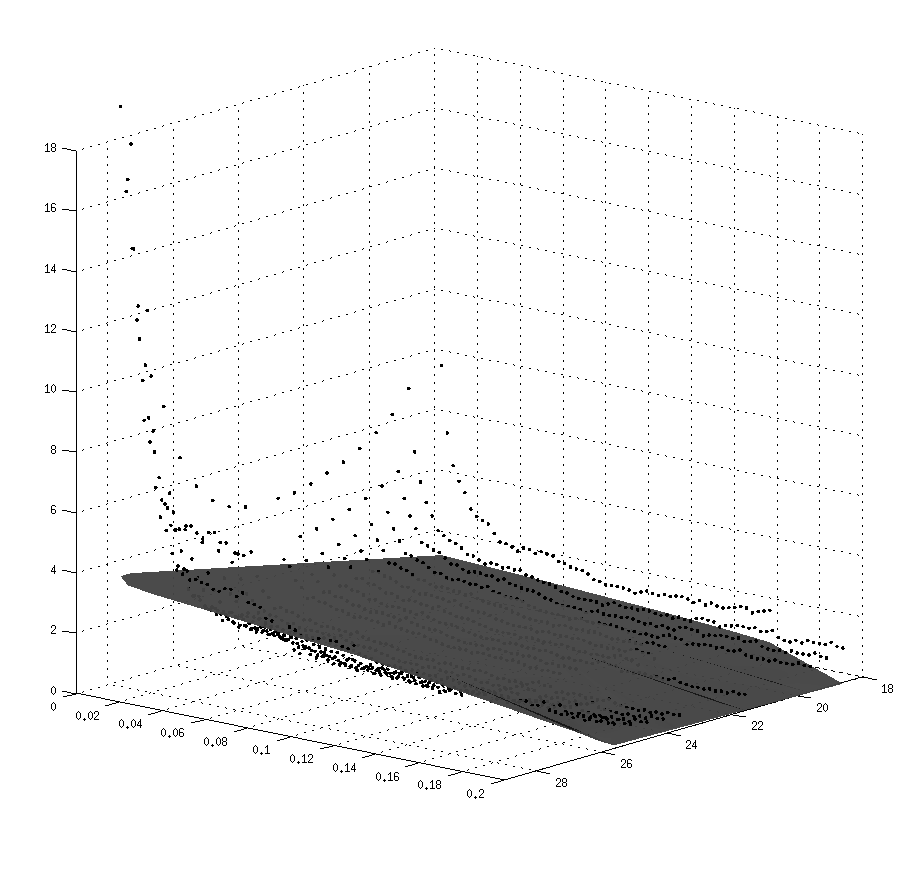
\includegraphics[width=8cm]{1.eps}
\end{multicols}

\hrule
\vspace{1cm}
Model\;2: $f(w,\mathbf{x})=(w*(x_1)^2+w*(x_1)+w)*(w*(x_2)^2+w*(x_2)+w)$

\begin{multicols}{2}
\begin{bundle}{times2}\chunk{\begin{bundle}{parabola}\chunk{x1}\end{bundle}}\chunk{\begin{bundle}{parabola}\chunk{x2}\end{bundle}}\end{bundle}

\columnbreak
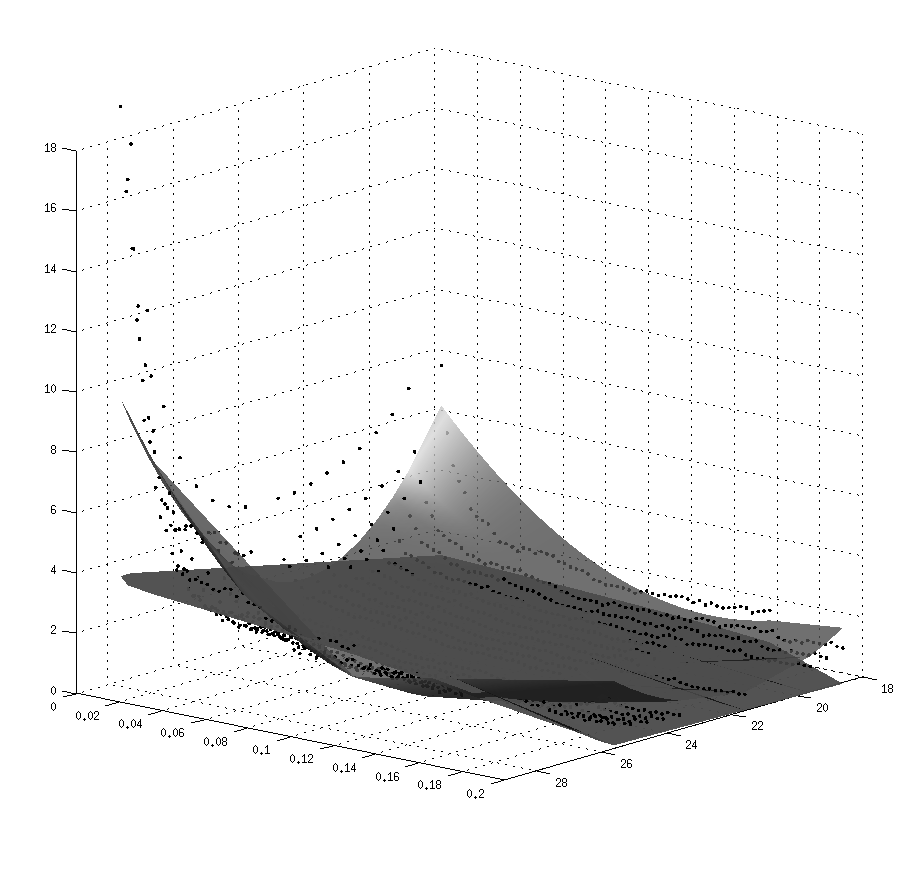
\includegraphics[width=8cm]{2.eps}
\end{multicols}

\hrule
\vspace{1cm}
Model\;3: $f(w,\mathbf{x})=(w+w*(x_1)+w*(e(x_1)*(x_1)p(w*(x_1)*(x_1))))*((w*(x_2)^2+w*(x_2)+w)*(w*(x_2)+w))$

\begin{multicols}{2}
\begin{bundle}{times2}\chunk{\begin{bundle}{plus}\chunk{\begin{bundle}{plus2}\chunk{\begin{bundle}{mult}\chunk{x1}\end{bundle}}\chunk{\begin{bundle}{mult}\chunk{\begin{bundle}{expl}\chunk{\begin{bundle}{times2}\chunk{x1}\chunk{x1}\end{bundle}}\end{bundle}}\end{bundle}}\end{bundle}}\end{bundle}}\chunk{\begin{bundle}{times2}\chunk{\begin{bundle}{parabola}\chunk{x2}\end{bundle}}\chunk{\begin{bundle}{linear}\chunk{x2}\end{bundle}}\end{bundle}}\end{bundle}

\columnbreak
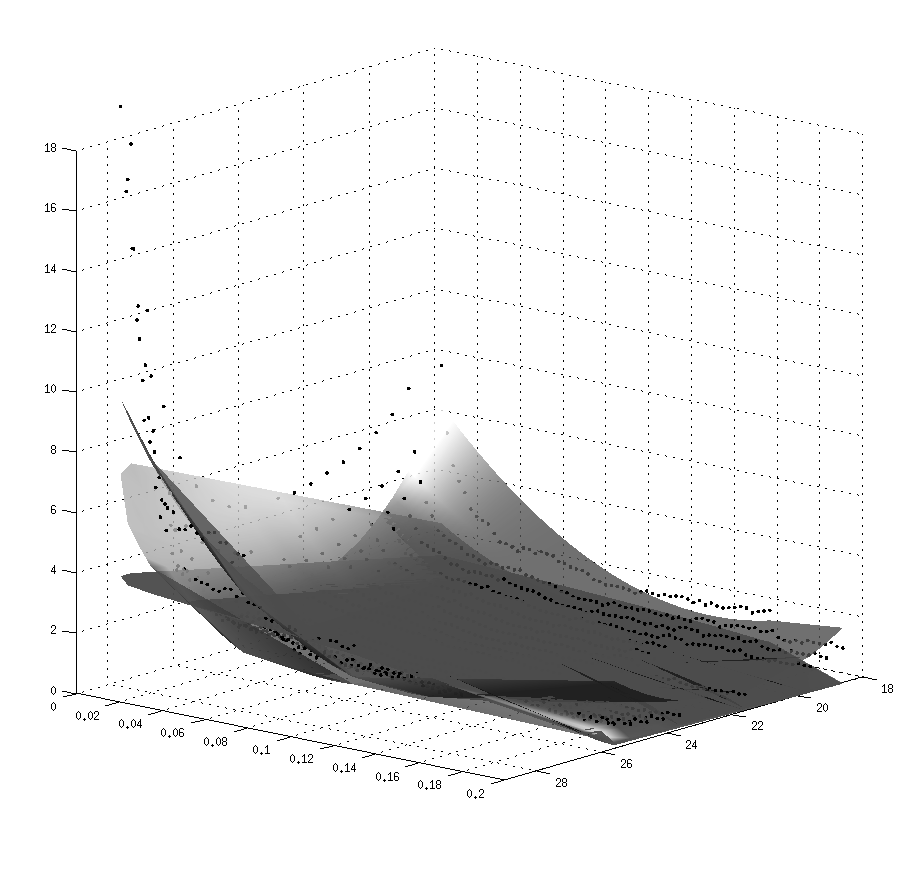
\includegraphics[width=8cm]{3.eps}
\end{multicols}

\hrule
\vspace{1cm}
Model\;4: $f(w,\mathbf{x})=(w*(sqrt(w*frac{w}{x_2}+w))^2+w*(sqrt(w*frac{w}{x_2}+w))+w)*(((sqrt(w*w*esin(w*x_1+w)p(((sin(w*x_1+w)-w)^2)*w)+w))*(x_1))*(frac{1}{1+efrac{1}{x_2}p(-frac{1}{x_2})}))$

\begin{multicols}{2}
\begin{bundle}{times2}\chunk{\begin{bundle}{parabola}\chunk{\begin{bundle}{sqrta}\chunk{\begin{bundle}{hyperbola}\chunk{x2}\end{bundle}}\end{bundle}}\end{bundle}}\chunk{\begin{bundle}{times2}\chunk{\begin{bundle}{times2}\chunk{\begin{bundle}{sqrta}\chunk{\begin{bundle}{normal}\chunk{\begin{bundle}{sina}\chunk{x1}\end{bundle}}\end{bundle}}\end{bundle}}\chunk{x1}\end{bundle}}\chunk{\begin{bundle}{logsig}\chunk{\begin{bundle}{inv}\chunk{x2}\end{bundle}}\end{bundle}}\end{bundle}}\end{bundle}

\columnbreak
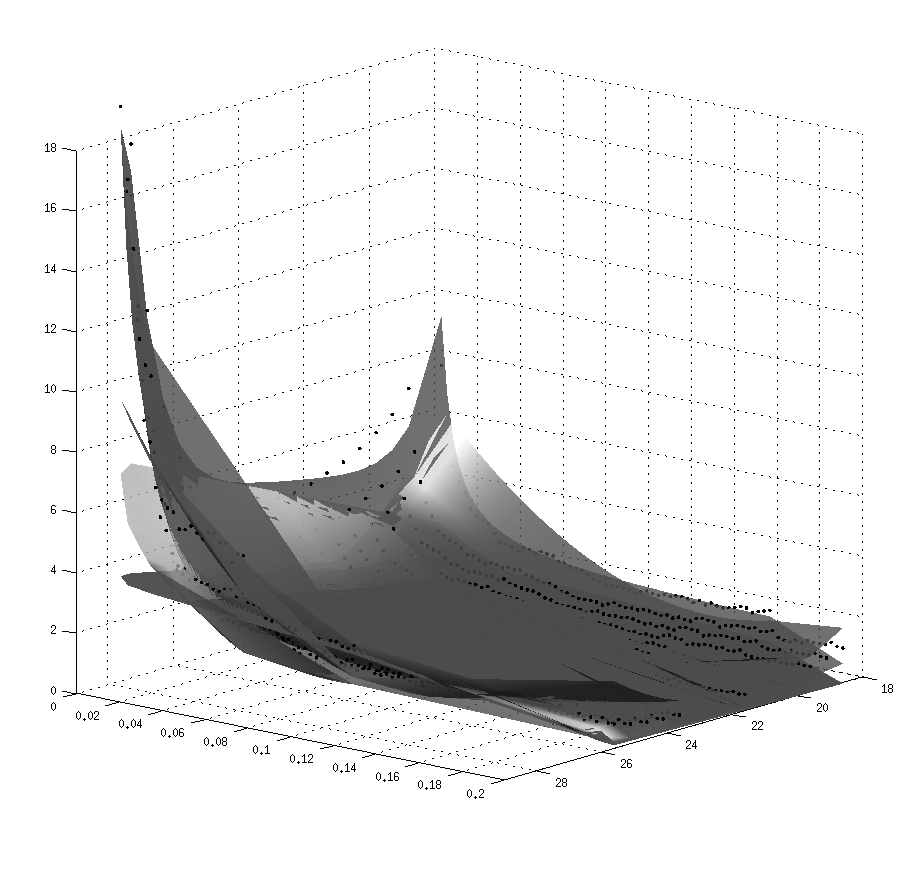
\includegraphics[width=8cm]{4.eps}
\end{multicols}

\hrule
\vspace{1cm}
Model\;5: $f(w,\mathbf{x})=(w+frac{1}{w*ex_2p(((x_2-w)^2)*w)}+sin(w*x_1+w))*((w*(sin(w*w*(x_2)+w+w))^2+w*(sin(w*w*(x_2)+w+w))+w)*(sqrt(w*x_2+w)))$

\begin{multicols}{2}
\begin{bundle}{times2}\chunk{\begin{bundle}{plus}\chunk{\begin{bundle}{plus2}\chunk{\begin{bundle}{inv}\chunk{\begin{bundle}{normal}\chunk{x2}\end{bundle}}\end{bundle}}\chunk{\begin{bundle}{sina}\chunk{x1}\end{bundle}}\end{bundle}}\end{bundle}}\chunk{\begin{bundle}{times2}\chunk{\begin{bundle}{parabola}\chunk{\begin{bundle}{sina}\chunk{\begin{bundle}{linear}\chunk{x2}\end{bundle}}\end{bundle}}\end{bundle}}\chunk{\begin{bundle}{sqrta}\chunk{x2}\end{bundle}}\end{bundle}}\end{bundle}

\columnbreak
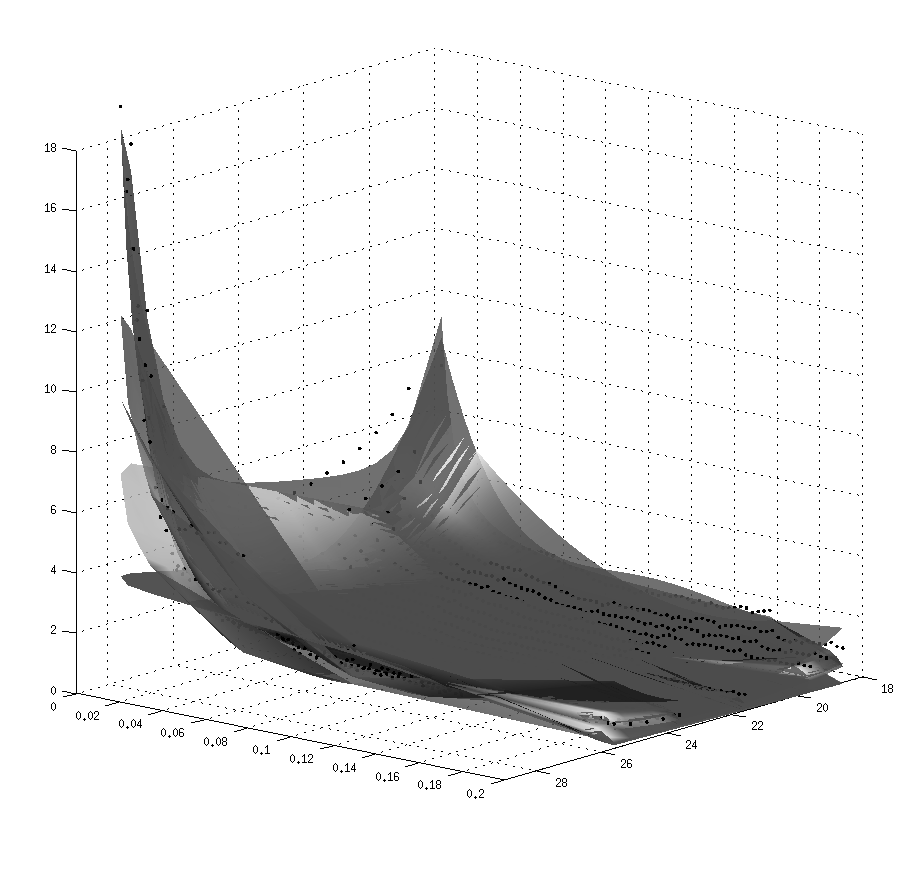
\includegraphics[width=8cm]{5.eps}
\end{multicols}

\hrule
\vspace{1cm}
Model\;6: $f(w,\mathbf{x})=((w*(sin(w*sin(w*w*(sqrt(x_1))+w+w)+w))^2+w*(sin(w*sin(w*w*(sqrt(x_1))+w+w)+w))+w)*(sqrt(w*frac{w}{x_2}+w)))*(w+sin(w*x_1+w)+x_2)$

\begin{multicols}{2}
\begin{bundle}{times2}\chunk{\begin{bundle}{times2}\chunk{\begin{bundle}{parabola}\chunk{\begin{bundle}{sina}\chunk{\begin{bundle}{sina}\chunk{\begin{bundle}{linear}\chunk{\begin{bundle}{sqrt}\chunk{x1}\end{bundle}}\end{bundle}}\end{bundle}}\end{bundle}}\end{bundle}}\chunk{\begin{bundle}{sqrta}\chunk{\begin{bundle}{hyperbola}\chunk{x2}\end{bundle}}\end{bundle}}\end{bundle}}\chunk{\begin{bundle}{plus}\chunk{\begin{bundle}{plus2}\chunk{\begin{bundle}{sina}\chunk{x1}\end{bundle}}\chunk{x2}\end{bundle}}\end{bundle}}\end{bundle}

\columnbreak
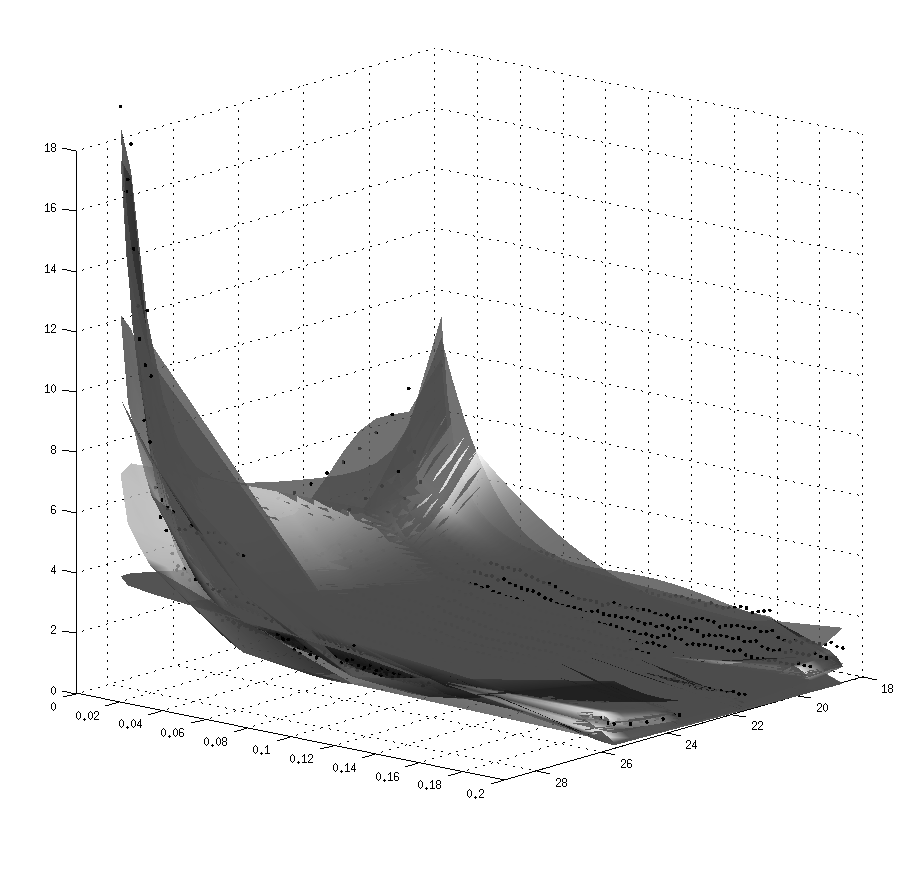
\includegraphics[width=8cm]{6.eps}
\end{multicols}

\end{document}